%\modeCorrection

%%%% début de la page
\renewcommand{\thesection}{\textcolor{red}{Partie \Roman{section} -}}
\renewcommand{\thesubsection}{\textcolor{red}{\Roman{section}.\arabic{subsection}}}
\renewcommand{\thesubsubsection}{\textcolor{red}{\Roman{section}.\arabic{subsection}.\alph{subsubsection}}}

\setcounter{section}{0}
\setcounter{document}{0}
\sndEnTeteTPDix

\begin{center}
\begin{mdframed}[style=titr, leftmargin=60pt, rightmargin=60pt, innertopmargin=7pt, innerbottommargin=7pt, innerrightmargin=8pt, innerleftmargin=8pt]

\begin{center}
\large{\textbf{TP 10 : L'apparition d'un arc-en-ciel
}}
\end{center}
\end{mdframed}
\end{center}

\begin{tableauCompetences}
    REA & Réaliser un montage à l'aide d'un protocole expérimental & & & & \\
    \hline
    APP & Exploiter un spectre d'émission & & & & \\   
    \hline 
    REA & Connaître et exploiter les lois de Snell-Descartes & & & & \\
    \hline 
    COM & Rendre compte de façon écrite & & & & \\
    \hline
    VAL & Analyser l’ensemble des résultats de façon critique  & & & &
\end{tableauCompetences}


%%%% objectifs
\begin{tcolorbox}[colback=blue!5!white,colframe=blue!75!black,title=Objectifs de la séance :]
\begin{itemize}
    \item Décrire et expliquer qualitativement le phénéomène de dispersion de la lumière par un prisme ;
    \item Produire et exploiter des spectres d'émission obtenus à l'aide d'un système dispersif et d'un analyseur de spectre ;
\end{itemize}
\end{tcolorbox}

%%%% Consignes
\begin{tcolorbox}[colback=red!5!white,colframe=red!75!black,title= Consignes :]
\begin{itemize}
    \item Faire attention au matériel lors de son utilisation ;
    \item Produire et rendre un compte rendu écrit de TP par binôme ;
\end{itemize}
\end{tcolorbox}

%%%% contexte
\section{Mise en évidence expérimentale}
\begin{tcolorbox}[colback=orange!5!white,colframe=orange!75!black,title= Expérience d'Isaac Newton :]
\begin{wrapfigure}{r}{0.4\textwidth}
%\vspace{-0.6cm}
    \centering
     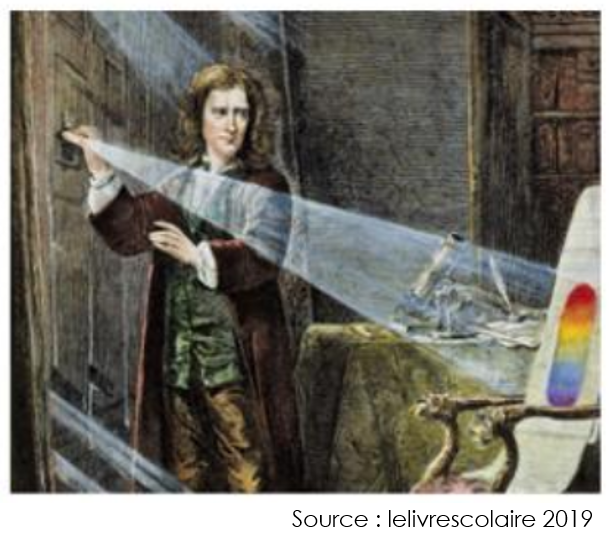
\includegraphics[width=0.4\textwidth]{Images/TP/TP10/Isaac_Newton.PNG}
   \end{wrapfigure}
Le physicien Isaac Newton (1643-1727) a mené en 1666 une expérience sur la lumière du Soleil qui allait révolutionner la conception de l'optique que l'on avait à l'époque. Pour cela, il a réalisé une petite ouverture dans son volet afin qu'un fin faisceau lumineux pénètre dans la pièce. Il a alors placé un prisme de verre sur le trajet de la lumière. Il a constaté que la lumière était déviée par le prisme et qu'elle formait sur un écran un dégradé de couleurs allant du rouge au violet, appelé \textcolor{red}{spectre}.\\

\problematique{Quel phénomène permet d'expliquer l'apparition d'un arc-en-ciel ?}
\end{tcolorbox}

\begin{mdframed}[style=autreexo]
\textbf{\bsc{Liste du matériel}}
\begin{multicols}{2}
    \begin{itemize}
    \item Un générateur de tension continue ;
    \item Une lampe à incandescence ;
    \item Une lentille convergente ;
    \item Une fente ;
    \item Un prisme ;
    \item Un écran ;
    \item Une lampe à vapeur de mercure ;
    \item Un filtre rouge et un filtre bleu ;
\end{itemize}
\end{multicols}
\end{mdframed}

\begin{large}
    \textbf{\textcolor{red}{\underline{Travail à réaliser :}}}
\end{large}
\\
\question{\`{A} l'aide du matériel que vous avez à disposition, réaliser la même expérience qu'Isaac Newton. Observe-t'on le même résultat que le physicien ?}{~}{0}
%\\
\question{Réaliser un schéma de votre expérience en reproduisant le résultat obtenu.}{~}{0}
%\\
\question{\`{A} l'aide du matériel que vous avez à disposition, réaliser la même expérience qu'Isaac Newton. }{~}{0}
\question{Mettre un filtre rouge devant la sortie de la lampe à incandescence. Réaliser la même expérience avec un filtre bleu. Reproduire le résultat sur un schéma pour chacune des expériences.}{}{0}
%\\
\question{Lorsque la lumière blanche traverse le prisme, quelle est la radiation la plus déviée ? La moins déviée ?}{~}{0}
%%%% documents

%%%%
\section{Exploitation des résultats}

\begin{doc}{Variation de l'indice optique du verre en fonction de la radiation qui le traverse}
    L'indice optique du verre dépend de la longueur d'onde de la radiation qui le traverse : un verre est un milieu dit \textcolor{red}{dispersif}. Par exemple, pour une radiation rouge, l'indice optique $n_{rouge}=1,510$ et pour une radiation bleue $n_{bleu}=1,520$.
\end{doc}
\begin{large}
    \textbf{\textcolor{red}{\underline{Travail à réaliser :}}}
\end{large}
\\
%\\

\question{Voici un prisme dont l'angle au sommet A vaut 35$\degree$ :
\begin{center}
    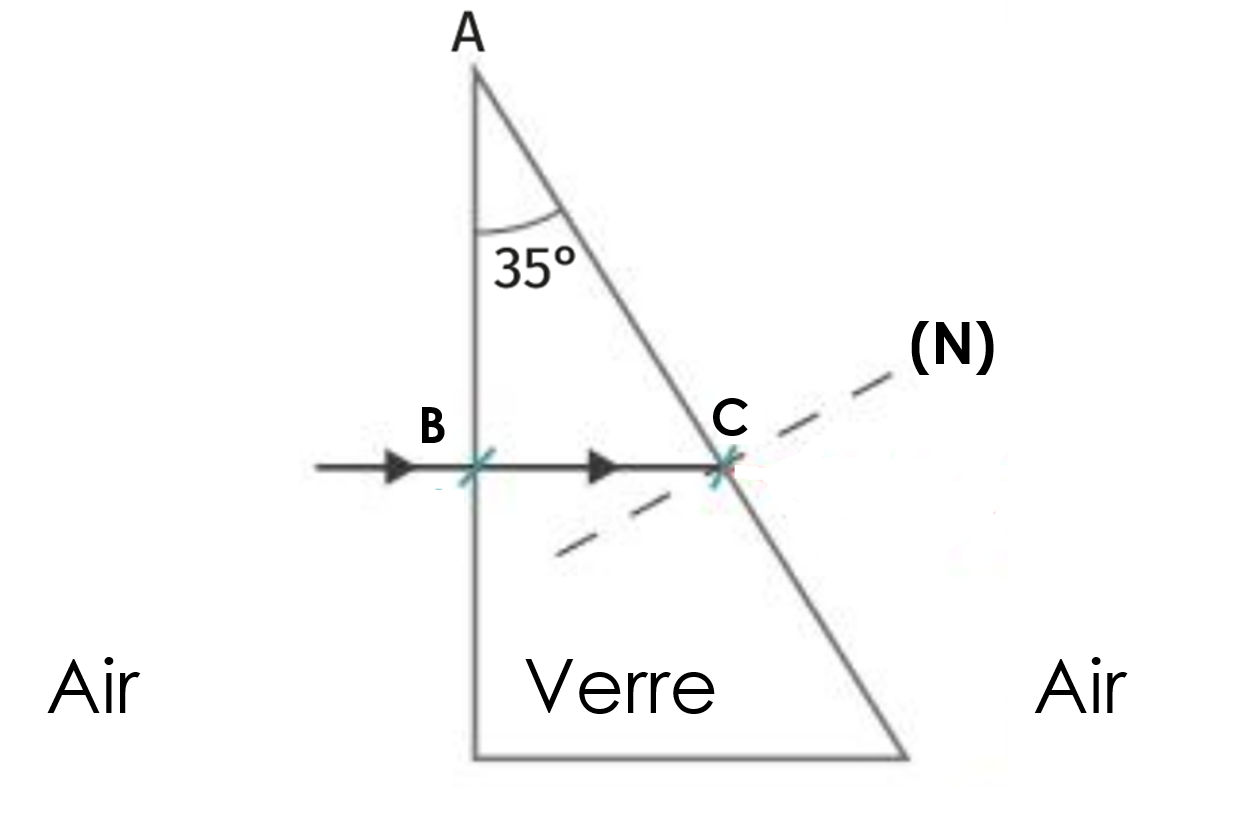
\includegraphics[scale=0.6]{Images/TP/TP10/Prisme_exo.PNG}
\end{center}
}{}{0}
\begin{minipage}{0.47\textwidth}
\question{Rappeler la loi de Snell-Descartes pour la réfraction.}{}{0}
%\\
\question{Justifier que le rayon n'est pas dévié au point I$_1$.}{L'angle d'incidence au point I$_1$ vaut $0\degree$, l'angle de réfraction est donc nul d'après la loi de Descartes sur la réfraction.}{0}
%\\
\question{Déterminer l'angle de réfraction de la lumière bleue en sachant que l'angle d'incidence au point I$_2$ vaut 35$\degree$.}{~}{0}

\end{minipage}
\hspace{0.05\textwidth}
\begin{minipage}{0.47\textwidth}

\end{minipage}
\hspace{0.05\textwidth}
\begin{minipage}{0.3\textwidth}

\end{minipage}

%\newpage
%\papiermillimetre